\begin{tikzpicture}
	\node at (0, 2) {\bfseries \small Quantum prior generation};
	\node at (0, 0) {\input{tikz/qcultrasimple}};
	\node (conv) at (6, 0.0) {\scalebox{.75}{\input{tikz/convhead}}};
	\draw[
	-{Triangle[width=16pt, length=16pt]},
	line width=12pt,
	color=\tertiarycolor!20
	] ([xshift=-1.5cm, yshift=0.5cm]conv.east) -- ++(1.5, 0);
	\node at ([xshift=2cm, yshift=.25cm]conv.east) {\scalebox{.4}{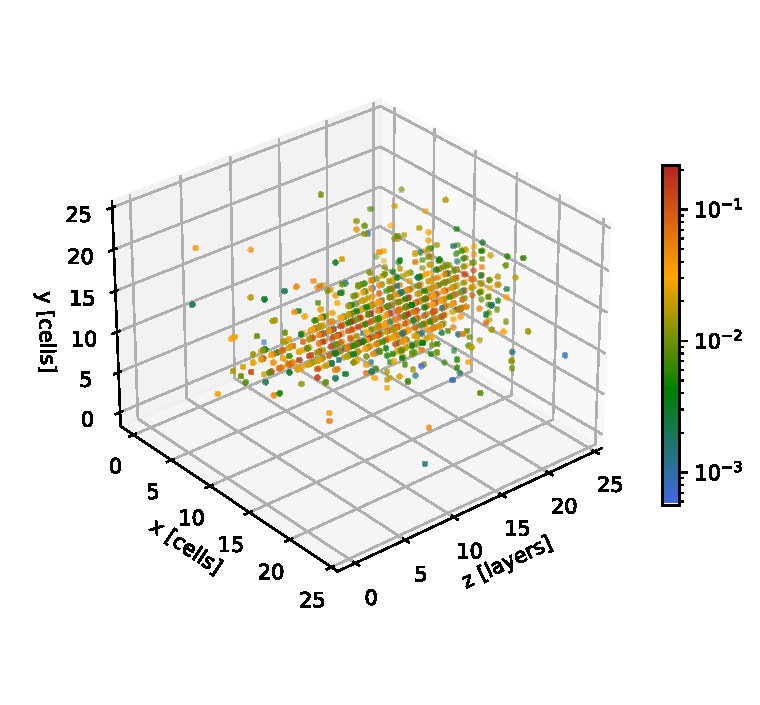
\includegraphics{assets/shower_example}}};

	\draw[black] ([xshift=5cm, yshift=-1.75cm]conv.east) -- ++(0, 4.5);

	\node[text width=6cm] at ([xshift=8cm, yshift=.5cm]conv.east) {
		\rule{.25cm}{0pt}\textbf{Training process:}
		\begin{itemize}
			\item Definition of Quantum Prior and Convoluting head;
			\item Propagate Observables through Circuit;
			\item Alterante Training: Prior + Classical head.
		\end{itemize}
	};

	\draw[
		black,
		line width=0.8pt,
		rounded corners=4pt
	]
	([xshift=0cm, yshift=.25cm]current bounding box.south west)
	rectangle
	([xshift=.25cm, yshift=.25cm]current bounding box.north east);

	\node[anchor=west] at ([xshift=.25cm, yshift=-.35cm]current bounding box.north west) {\bfseries C: Hybrid Model + Pauli Propagation};

\end{tikzpicture}